\documentclass[a4paper,10pt]{scrartcl}
\usepackage[utf8]{inputenc}

% Title Page
\title{Lectures ?--?: Numerical Methods}
\author{Andrew D. Wickert}
\date{Last updated \today}

\usepackage{listings}
\usepackage{color}
%\usepackage{url}
\usepackage[colorlinks=true]{hyperref}

\usepackage{amssymb}
\usepackage{amsmath}
\usepackage{graphicx}

\newcommand{\todo}[1]{\textcolor{red}{@TODO: #1}} 
 
% From http://en.wikibooks.org/wiki/LaTeX/Source_Code_Listings, modified a little

\definecolor{mygreen}{rgb}{0,0.6,0}
\definecolor{mygray}{rgb}{0.5,0.5,0.5}
\definecolor{mymauve}{rgb}{0.58,0,0.82}

\lstset{ %
  backgroundcolor=\color{white},   % choose the background color; you must add \usepackage{color} or \usepackage{xcolor}
  basicstyle=\scriptsize,          % the size of the fonts that are used for the code
  breakatwhitespace=false,         % sets if automatic breaks should only happen at whitespace
  breaklines=true,                 % sets automatic line breaking
  captionpos=b,                    % sets the caption-position to bottom
  commentstyle=\color{mygreen},    % comment style
  deletekeywords={...},            % if you want to delete keywords from the given language
  escapeinside={\%*}{*)},          % if you want to add LaTeX within your code
  extendedchars=true,              % lets you use non-ASCII characters; for 8-bits encodings only, does not work with UTF-8
  frame=single,                    % adds a frame around the code
  keepspaces=true,                 % keeps spaces in text, useful for keeping indentation of code (possibly needs columns=flexible)
  keywordstyle=\color{blue},       % keyword style
  language=Python,                 % the language of the code
  morekeywords={*,...},            % if you want to add more keywords to the set
  numbers=left,                    % where to put the line-numbers; possible values are (none, left, right)
  numbersep=5pt,                   % how far the line-numbers are from the code
  numberstyle=\tiny\color{mygray}, % the style that is used for the line-numbers
  rulecolor=\color{black},         % if not set, the frame-color may be changed on line-breaks within not-black text (e.g. comments (green here))
  showspaces=false,                % show spaces everywhere adding particular underscores; it overrides 'showstringspaces'
  showstringspaces=false,          % underline spaces within strings only
  showtabs=false,                  % show tabs within strings adding particular underscores
  stepnumber=2,                    % the step between two line-numbers. If it's 1, each line will be numbered
  stringstyle=\color{mymauve},     % string literal style
  tabsize=2,                       % sets default tabsize to 2 spaces
  title=\lstname                   % show the filename of files included with \lstinputlisting; also try caption instead of title
}

\begin{document}
\maketitle

\section{Mathematics Review}

\subsection{Derivatives}

A derivative is the change in a function ($f(x)$) with respect to the change in the independent variable ($x$) as the interval ($\Delta x$) approaches 0:

\begin{equation}
 \frac{d}{{dx}}f\left( x \right) = \mathop {\lim }\limits_{\Delta x \to 0} \frac{{f\left( {x + \Delta x } \right) - f\left( x \right)}}{\Delta x }
\end{equation}

\begin{figure}[!ht]
\begin{center}
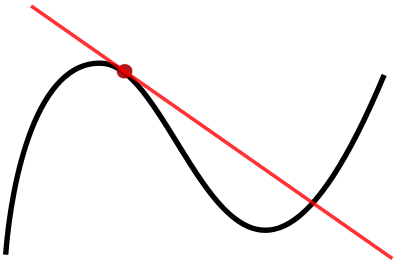
\includegraphics[width=.5\linewidth]{figures/NumericalAndMath/400px-Tangent_to_a_curve.png}
\end{center}
\caption{The graph of a function, drawn in black, and a tangent line to that function, drawn in red. The slope of the tangent line is equal to the derivative of the function at the marked point. (Text from \url{https://en.wikipedia.org/wiki/Derivative} on 2015.05.07; borrowing it because I couldn't find a better way to say it!)}
\end{figure}

\todo{Create a better figure for derivative definition and finite difference, with shown $\Delta x$}

\subsection{Integrals}

Integration 
An indefinite integral 



\begin{equation}
\int_a^b \! f(x)\,dx = F(b) - F(a)
\end{equation}

\begin{equation}
\int_a^b \! f(x)\,dx
\end{equation}

\begin{figure}[!ht]
\begin{center}
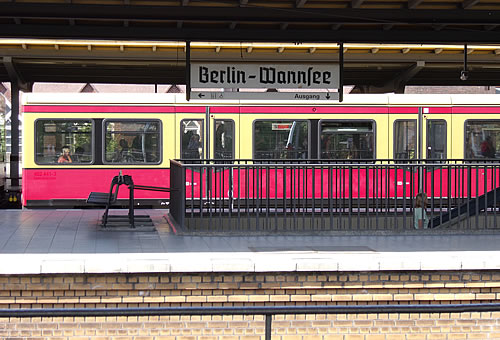
\includegraphics[width=.5\linewidth]{figures/NumericalAndMath/BerlinWannsee.jpg}
\end{center}
\caption{This ``S'' in the Berlin--Wannsee station sign is written in the old style. It is used for integrals to stand for ``sum'', as the area under a curve can be imagined to be a sum $\left( \sum \right)$ of every infinitessimally thin column of space under a curve.}
\end{figure}

\begin{figure}[!ht]
\begin{center}
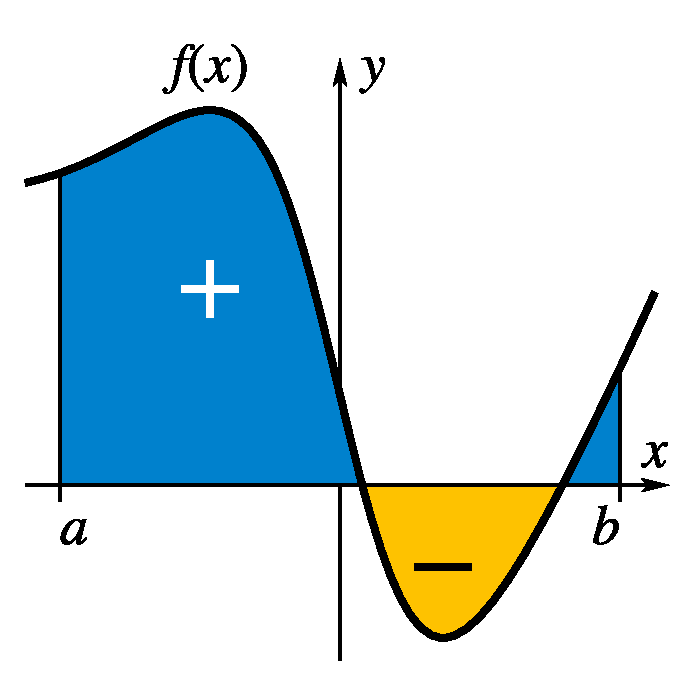
\includegraphics[width=.5\linewidth]{figures/NumericalAndMath/IntegralExample.pdf}
\end{center}
\caption{An integral is the sum of all area under a curve. (Contributed to Wikimedia Commons by User:KSmrq)}
\end{figure}


\subsection{Taylor series}

The Taylor series of any complex function $f(x)$ (i.e., $f(x) \in \mathbb{C}$) that is infinitely differentiable at a point $x_0$ approximates that function as a power series:
\begin{equation}
f(x_0)+\frac {f'(x_0)}{1!} (x-x_0)+ \frac{f''(x_0)}{2!} (x-x_0)^2+\frac{f^{(3)}(x_0)}{3!}(x-x_0)^3+ \cdots
\end{equation}
Or, in the more-compact summation notation, this is:
\begin{equation}
\sum_{n=0} ^ {\infty} \frac {f^{(n)}(x_0)}{n!} \, (x-x_0)^{n}
\end{equation}
where $n$ is the number of the derivative of $f$.

\begin{figure}[!ht]
\begin{center}
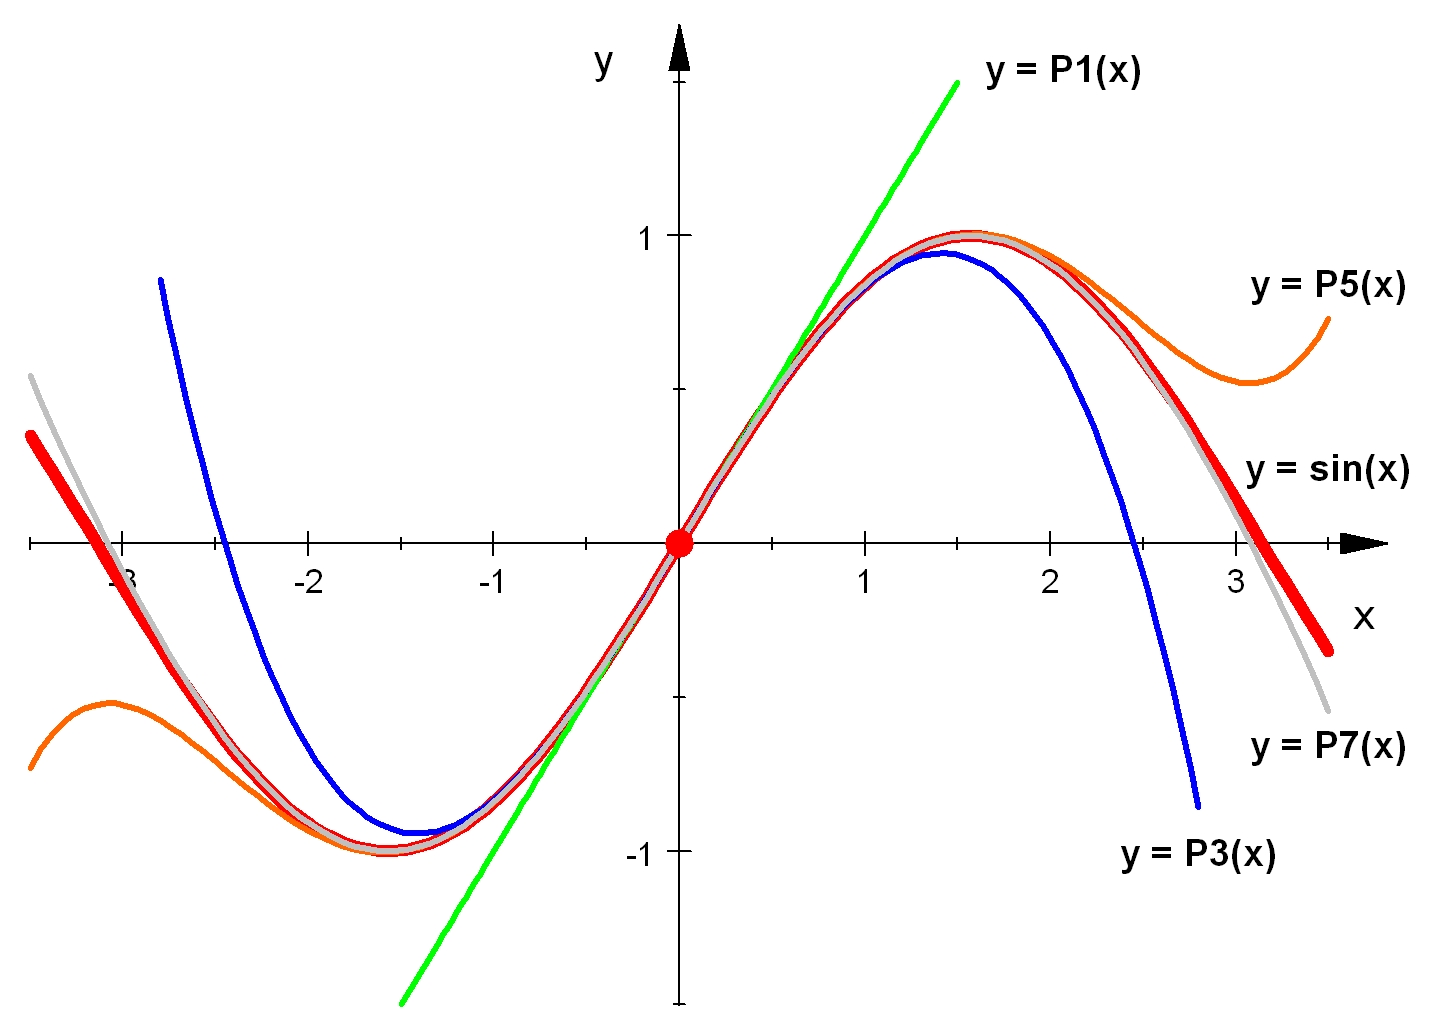
\includegraphics[width=.8\linewidth]{figures/NumericalAndMath/Taylor_Approximation_of_sin(x).jpeg}
\end{center}
\caption{Increasing orders of the derivative $n$, denoted P$n$, where $n = 1, 2, 3, \cdots$, show the increasing approximation of a sum of polynomials to the sine function.}
\end{figure}



dot products

cross products

vectors

tensors


Meshes

\section{Finite difference}

\subsection{Discretization}

You may have wondered why I covered derivatives and Taylor series right after one another

Finite difference, finite element, and spectral

Forward difference and ``implicit''
on both structured and unstructured meshes

Stencils

Linearizing equations (is this the right word? turning them into a set of linear equations)

Differential equations and linear algebra review

Include examples

\end{document}          
